\section{\acs{5G} Resource Lifecycle Management}
\label{chap:impl:resource_lifecycle}

As established in Section~\ref{chap:proposal:resource_lifecycle}, network slicing is the main mechanism that allows the testbed to support diverse vertical use cases and network applications, and their respective heterogeneous \acs{QoS} requirements. Delivering this requires the automation and orchestration of each phase of the \acs{NSI} lifecycle, a responsibility handled by the coordinated operation of the \acs{CSMF}, \acs{NSMF} and \acs{NSSMF} management functions. In this section, the components responsible for realizing each of these management functions are identified. However, in practice, not all of these functions have a direct counterpart within the implementation developed in this dissertation, being instead abstracted by other components already present in the \acs{ITAv} 5GAIner testbed~\cite{5GAIner}.

At the top of this management hierarchy, the \acs{OSL} \acs{OSS}~\cite{OpenSlice} is responsible for the \acs{OAM} functionality within the testbed, fulfilling the \acs{CSMF} role established in Section~\ref{chap:proposal:resource_lifecycle}. In this capacity, it exposes communication services to third-party clients through \acs{TMF} Open \acsp{API}, allowing them to request and provision \acs{5G} resources (network slices and \acsp{UE}) without requiring privileged knowledge of the underlying infrastructure. This abstraction is implemented by leveraging the \acf{CFS}, \acf{RFS} and Resource constructs, defined by \acs{TMF}, as mentioned in Section~\ref{sota:telcoinitiatives:tmf}. More concretely, each \acs{CFS} is exposed to customers as a configurable interface, through which clients can specify their desired service parameters (e.g. uplink throughput for a slice). Internally, the fields of the \acs{CFS}, expressing the user's requirements, are then mapped into a corresponding \acs{RFS} which in turn references the concrete Resource capturing the technical parameters required to provision the underlying network slice or \acs{UE}.

However, as previously discussed, \acs{OSL} is not an orchestrator, meaning the provisioning of the resources referenced by each \acs{RFS} is delegated to dedicated components. Therefore, \acs{OSL}, can delegate the provisioning of \acs{NFV} resources, to \acs{NFV} \acs{OSM}, via the SOL005 interface. Containerized resources, such as network applications, can also be automatically deployed to kubernetes through the CRIDGE component. In the case of network slices and \acsp{UE}, the provisioning of resources is delegated to a proprietary Slice Manager within \acs{ITAv}'s testbed.

This proprietary Slice Manager represents the primary mechanism for interacting with the \acs{5G} System, both the \acs{RAN} and the core, to provision network slices and \acsp{UE} in the 5GAIner infrastructure. This component abstracts the underlying complexity of interacting with the \acs{5G} System and \acs{NFV} infrastructure behind a unified \acs{API}, simplifying the management of \acs{5G} resources. Given the abstraction provided by this \acs{API}, the design and implementation of the \acs{NSMF} and \acs{NSSMF} services falls outside the scope of this dissertation, as their underlying functionality is already encapsulated within the Slice Manager. Consequently, \acs{OSL} must be capable of converting high-level customer service requirements, provided via a \acs{CFS}, into concrete \acs{API} calls to the Slice Manager, resulting in the provisioning of network slices and \acsp{UE}. This can be accomplished through the use of \acs{OSL} Generic Controllers~\cite{OpenSliceGenericServicesController}, which will be discussed in detail in the next section.

\subsection{Slicing Generic Controller}
\label{chap:impl:resource_lifecycle:controller}

A Generic Controller, inspired by the kubernetes operator pattern, is an \acs{OSL} component capable of managing resources of a specific type (of their resource specification)~\cite{OpenSliceGenericServicesController}. It is integrated natively into the OSL lifecycle, allowing custom code to be executed in response to the creation, update, and deletion of \acs{OSL} resources, by listening to a dedicated message queue for resource lifecycle events. This automated process allows the \acs{OSL} resources and services to be managed programmatically, ensuring they remain aligned with the state of the \acs{5G} deployment.

The Generic Controller\footnote{\url{https://github.com/Testbed-TNEI/SlicingGenericController}} developed in this dissertation was implemented using the Java Spring framework and manages two resource types: network slices and \acsp{UE}. For each resource type, a Resource Specification was defined, establishing the schema of the managed resource, aligned with the corresponding resource fields required by the Slice Manager \acs{API}. The controller runs as a standalone container, integrated with the \acs{OSL} deployment via its message queue. In this section, the design and implementation of the Generic Controller is presented, detailing how the controller converts the \acs{OSL} resource fields into Slice Manager \acs{API} calls for each resource type. It also describes how \acs{OSL} services are composed and structured into \acsp{CFS} and \acsp{RFS}, and addresses the integration of the testbed's observability mechanisms to monitor network slices and \acsp{UE} automatically upon provisioning.

\subsubsection{Network Slice Lifecycle Management}

The Slicing Generic Controller manages the lifecycle of network slice resources in the testbed. Each slice resource is defined by a Resource Specification capturing the parameters required for provisioning the resource using the Slice Manager \acs{API}. The required payload is provided in Appendix~\ref{appendix:slicemanager:payloads}, Code Block~\ref{code:slicemanager:payloads:netslice}, and its most relevant parameters include:

\begin{itemize}
    \item \texttt{id} \texttt{|} \texttt{name}: uniquely identify the slice resource in the \acs{5G} System;
    \item \texttt{administrative\_state} \texttt{|} \texttt{operational\_state}: indicate the slice status, regarding service (\texttt{LOCKED}, \texttt{UNLOCKED} or \texttt{SHUTTINGDOWN}) and operational state (\texttt{ENABLED} or \texttt{DISABLED}), respectively. The former controls whether the slice is available for use, while the latter its actual runtime condition and if it's capable of receiving traffic;
    \item \texttt{sst} \texttt{|} \texttt{ssd}: collectively form the \acs{S-NSSAI} identifier, classifying the slice type (e.g. \acs{eMBB}) and differentiating between slices of the same type, respectively;
    \item \texttt{dnn}: identifies the name of the target data network for the network slice;
    \item \texttt{dllatency} \texttt{|} \texttt{ullatency} \texttt{|} \texttt{dlguathptperue} \texttt{|} \texttt{ulguathptperue} \texttt{|} \texttt{dlmaxthpt\-perue} \texttt{|} \texttt{ulmaxthptperue} \texttt{|} \texttt{dlguathptperslice} \texttt{|} \texttt{ulguathptperslice} \texttt{|} \texttt{dl\-maxthptperslice} \texttt{|} \texttt{ulmaxthptperslice}: define the \acs{QoS} performance requirements of the slice, covering downlink and uplink latency, guaranteed and maximum throughput per \acs{UE}, and guaranteed and maximum throughput of the slice, respectively.
\end{itemize}

The fields of the Resource Specification, illustrated in Figure~\ref{} and defined in Code Block ~\ref{} (at Appendix~\ref{}), are aligned with the parameters accepted by the Slice Manager \acs{API}, allowing the Generic Controller to directly incorporate the resource state into the corresponding \acs{API} payload. Upon resource creation, the Generic Controller receives the  corresponding \texttt{CREATION} message and issues a \texttt{POST} request to the \texttt{/productOrder} endpoint of the Slice Manager \acs{API}, instantiating the network slice across the \acs{RAN} and \acs{CN}. Update events trigger a \texttt{PATCH} request to the \texttt{/productOrder/\{id\}/patch} endpoint of the Slice Manager \acs{API}, including the slice id and the modified resource parameters to update the slice configuration according to the new client requirements. Deletion of the resource triggers a \texttt{DELETE} request to the \texttt{/productOrder/\{id\}} endpoint of the Slice Manager \acs{API}, resulting in the deprovisioning of the slice and disassociation of any linked \acsp{UE}, operations that are once again abstracted by the Slice Manager component.

\subsubsection{\acl{UE} Lifecycle Management}

The Slicing Generic Controller also manages the lifecycle of \acs{UE} resources, handling their configuration, instantiation and association with the provisioned network slices. Following the same pattern established for the network slice resource, each \acs{UE} resource is defined by a Resource Specification with the exact parameters required by the Slice Manager \acs{API} to manage \acsp{UE}. The corresponding payload is also provided in Appendix~\ref{appendix:slicemanager:payloads}, Code Block~\ref{code:slicemanager:payloads:ue}, and its most relevant parameters include:

\begin{itemize}
    \item \texttt{IMSI}: identifies the \acs{UE} within the \acs{5G} network through its \acf{IMSI};
    \item \texttt{slice}: references the identifier of the network slice with which the \acs{UE} is to be associated, linking the device to the corresponding provisioned slice;
    \item \texttt{IPV4} \texttt{|} \texttt{IPV6}: define the \acs{IP} addresses assigned to the \acs{UE} within the target slice, used for traffic routing and \acs{UE} telemetry collection by the monitoring stack;
    \item \texttt{AMBRUP} \texttt{|} \texttt{AMBRDW}: optionally define the Aggregate Maximum Bit Rate of the \acs{UE} in the uplink and downlink directions, across non-\acs{GBR} sessions, respectively.
\end{itemize}

Following the same approach as in the network slice case, the \acs{UE} Resource Specification incorporates the same fields as those required by the corresponding Slice Manager \acs{API} requests, as showcased in Figure \ref{} (and Code Block~\ref{} at Appendix~\ref{}). Similarly, upon resource creation, the Generic Controller receives the corresponding \texttt{CREATION} message and issues a \texttt{POST} request to the \texttt{/ue/post} endpoint of the Slice Manager \acs{API}, registering the \acs{UE} and associating it with the target slice specified in the \texttt{slice} field. Deletion of the resource triggers a \texttt{DELETE} request to the \texttt{/ue/\{imsi\}/delete\_IMSI} endpoint, which simultaneously handles the removal of the \acs{UE} and its disassociation from the corresponding slice. However, the Slice Manager \acs{API} does not expose a dedicated endpoint for modifying a given \acs{UE}, which means that updating the slice association of an active \acs{UE} or any of its fields is not directly supported under the current implementation of the slicing generic controller. Consequently, any modification to an active \acs{UE}, including a change to its slice association, requires deleting and recreating the corresponding resource, knowing that in an optimal setting, it should be possible to migrate a \acs{UE} between slices without this overhead.

\subsection{Service Composition}

The Slicing Generic Controller, as any \acs{OSL} Generic Controller, manages the network slice and \acs{UE} entities at the resource level, representing the lowest layer of the \acs{TMF} hierarchy previously described, i.e. Product, Service and Resource. To make these resources configurable and available through the \acs{OSL} service layer and \acs{TMF} \acsp{API}, corresponding \acsp{RFS} are defined for each resource type, encapsulating the resource and inheriting all its fields as configurable parameters. By leveraging the Network Slice and \acs{UE}'s \acs{RFS}, presented in Figures \ref{} and \ref{}, operators or anyone designing services in \acs{OSL} possess all the means necessary to provision and manage network slices and the associated \acsp{UE}.

To expose these network slice and \acs{UE} management capabilities to third-party clients, \acsp{CFS} can be defined, namely a Network Slice \acs{CFS} and a UE \acs{CFS} composed by the corresponding \acsp{RFS}, each built on top of the respective \acsp{RFS}. This way, the service designer has control over which parameters are configurable through the \acs{CFS}, ensuring that only the fields relevant to the intended use case are exposed to customers. However, since \acs{CFS} and \acs{RFS} are distinct service constructs within \acs{OSL}, \acs{LCM} rules are required to keep them synchronized and ensure the \acs{OSL} state accurately reflects the state of the Slice Manager and, consequently, of the \acs{5G} System. Any changes to the customer requirements, defined via the \acs{OSL} \acs{CFS} fields, must be propagated downwards to the corresponding \acs{RFS} fields, triggering resource provisioning via the Generic Controller and corresponding Slice Manager \acs{API} call. Similarly, once the Slice Manager processes the request, the Generic Controller must update the corresponding resource fields based on the response, whether the operation was successful or not. In the event of a failure, this may involve rolling back the customer changes and displaying a user-friendly error message. The resulting state is then propagated upwards to the \acs{CFS} via \acs{LCM} rules, ensuring the \acs{OSL} service state remains consistent with the actual network state and that the result is reported back clearly to the user.

In this dissertation, three \acs{CFS} specifications are developed to address the management of network slices and \acsp{UE}, which are presented in Figure \ref{}. A standalone Network Slice \acs{CFS} and a standalone \acs{UE} \acs{CFS} are provided for the independent management of each resource type. Additionally, a bundled Network Slice and \acs{UE} \acs{CFS} groups the provisioning of a network slice and one associated \acs{UE} into a single service request. In both the Network Slice and Bundled \acs{CFS}, the network slice \texttt{id} is automatically generated (\acs{UUID}) by \acs{OSL}, before provisioning it through the Slice Manager \acs{API}. For the standalone \acs{UE} \acs{CFS}, the Generic Controller must additionally validate that the referenced network slice exists and that its maximum number of \acsp{UE} isn't exceeded by associating this additional \acs{UE}.


\subsection{Observability Integration}

As established in Section~\ref{chap:proposal:observability}, a core objective of the testbed is to deliver a fully automated monitoring process that can operate without manual human intervention. For this goal to be accomplished, the monitoring procedures must be directly integrated into the provisioning lifecycle managed by \acs{OSL}, ensuring that telemetry dashboards and/or collection are automatically enabled and disabled according to the lifecycle of each slice and \acs{UE} resource, and their parameters (e.g. \acs{UE} \acs{IP} or \acs{MAC} address). The underlying observability components responsible for collecting and exposing these metrics are described in detail in Section~\ref{chap:impl:observability}. This section focuses on how their integration is implemented with the developed Slicing Generic Controller and \acs{OSL}.

Once a network slice (service) is ordered in \acs{OSL}, a Grafana dashboard is automatically provisioned, scoped to that slice and its associated \acsp{UE}. This is achieved through a \texttt{PRE\_PROVISION} \acs{LCM} rule which triggers a Jenkins pipeline that deployes a Grafana Helm chart, pre-configured with a Prometheus data source (responsible for storing passive monitoring metrics of the \acs{5G} network) and the corresponding slice dashboards exposing the relevant metrics, as showcased in Figure \ref{}. As \acsp{UE} are subsequently associated with or disassociated from the slice (when deleted), the dashboard is updated accordingly, ensuring that the dashboard metrics always reflect the current set of \acsp{UE} assigned to the slice.

In Section~\ref{chap:proposal:observability:activemonitoring} active probing was introduce as a complement to passive monitoring. However, this monitoring approach continuously generates synthetic traffic targeting provisioned \acs{UE}, introducing additional load on the network. Therefore, it is not appropriate for it to be mandatory for every slice and \acs{UE}. Thus, active probing is only activated when the customer explicitly requests it, by setting the \texttt{active\_probing} field to \texttt{true} in the Network Slice \acs{CFS}. Internally, this results in the Generic Controller performing an \texttt{UPDATE} request to an \acs{API} endpoint encapsulating the prober configuration file, also described in Section~\ref{chap:impl:observability}.

Similarly to the approach discussed in the previous section, any changes to the \acs{OSL} services must also be reflected in the corresponding observability procedures. After provisioning a new slice and respective grafana dashboard, newly provisioned \acsp{UE} trigger the extension of that dashboard and, where applicable, the registration of their \acs{IP} addresses with the probing container. When the \acs{OSL} \acs{UE} resource is deleted and the \acs{UE} deprovisioned, the corresponding entries are removed from the slice dashboard and any active probing sessions terminated. Finally, upon deleting the slice, the corresponding dashboard and grafana deployment should be deprovisioned. Should any of these operations not complete as expected, the outcome must be reported back to the client, with the \acs{OSL} service state always reflecting the latest active monitoring configuration.

\subsection{Slicing Management Interaction Flow}

The previous sections described the network slice and \acs{UE} resources managed by the Slicing Generic Controller, as well as their composition into \acs{OSL} services. This section details how each resource lifecycle event received from \acs{OSL}, more specifically from its service orchestration and order management component (OSOM), is translated into the corresponding Slice Manager \acs{API} operations. 

The current version of the Slice Manager \acs{API} adopts an asynchronous processing model, in which each write operation is accepted immediately and assigned a unique operation identifier, used to subsequently retrieve the execution outcome. Figure~\ref{fig:impl:resource_lifecycle:flow:sequence} illustrates the interaction sequence between the \acs{OSL} orchestrator and \acs{TMF} \acsp{API}, the Slicing Generic Controller and the Slice Manager, for the creation, update and deletion of network slice and \acs{UE} resources.

\begin{figure}[htbp]
    \centering
    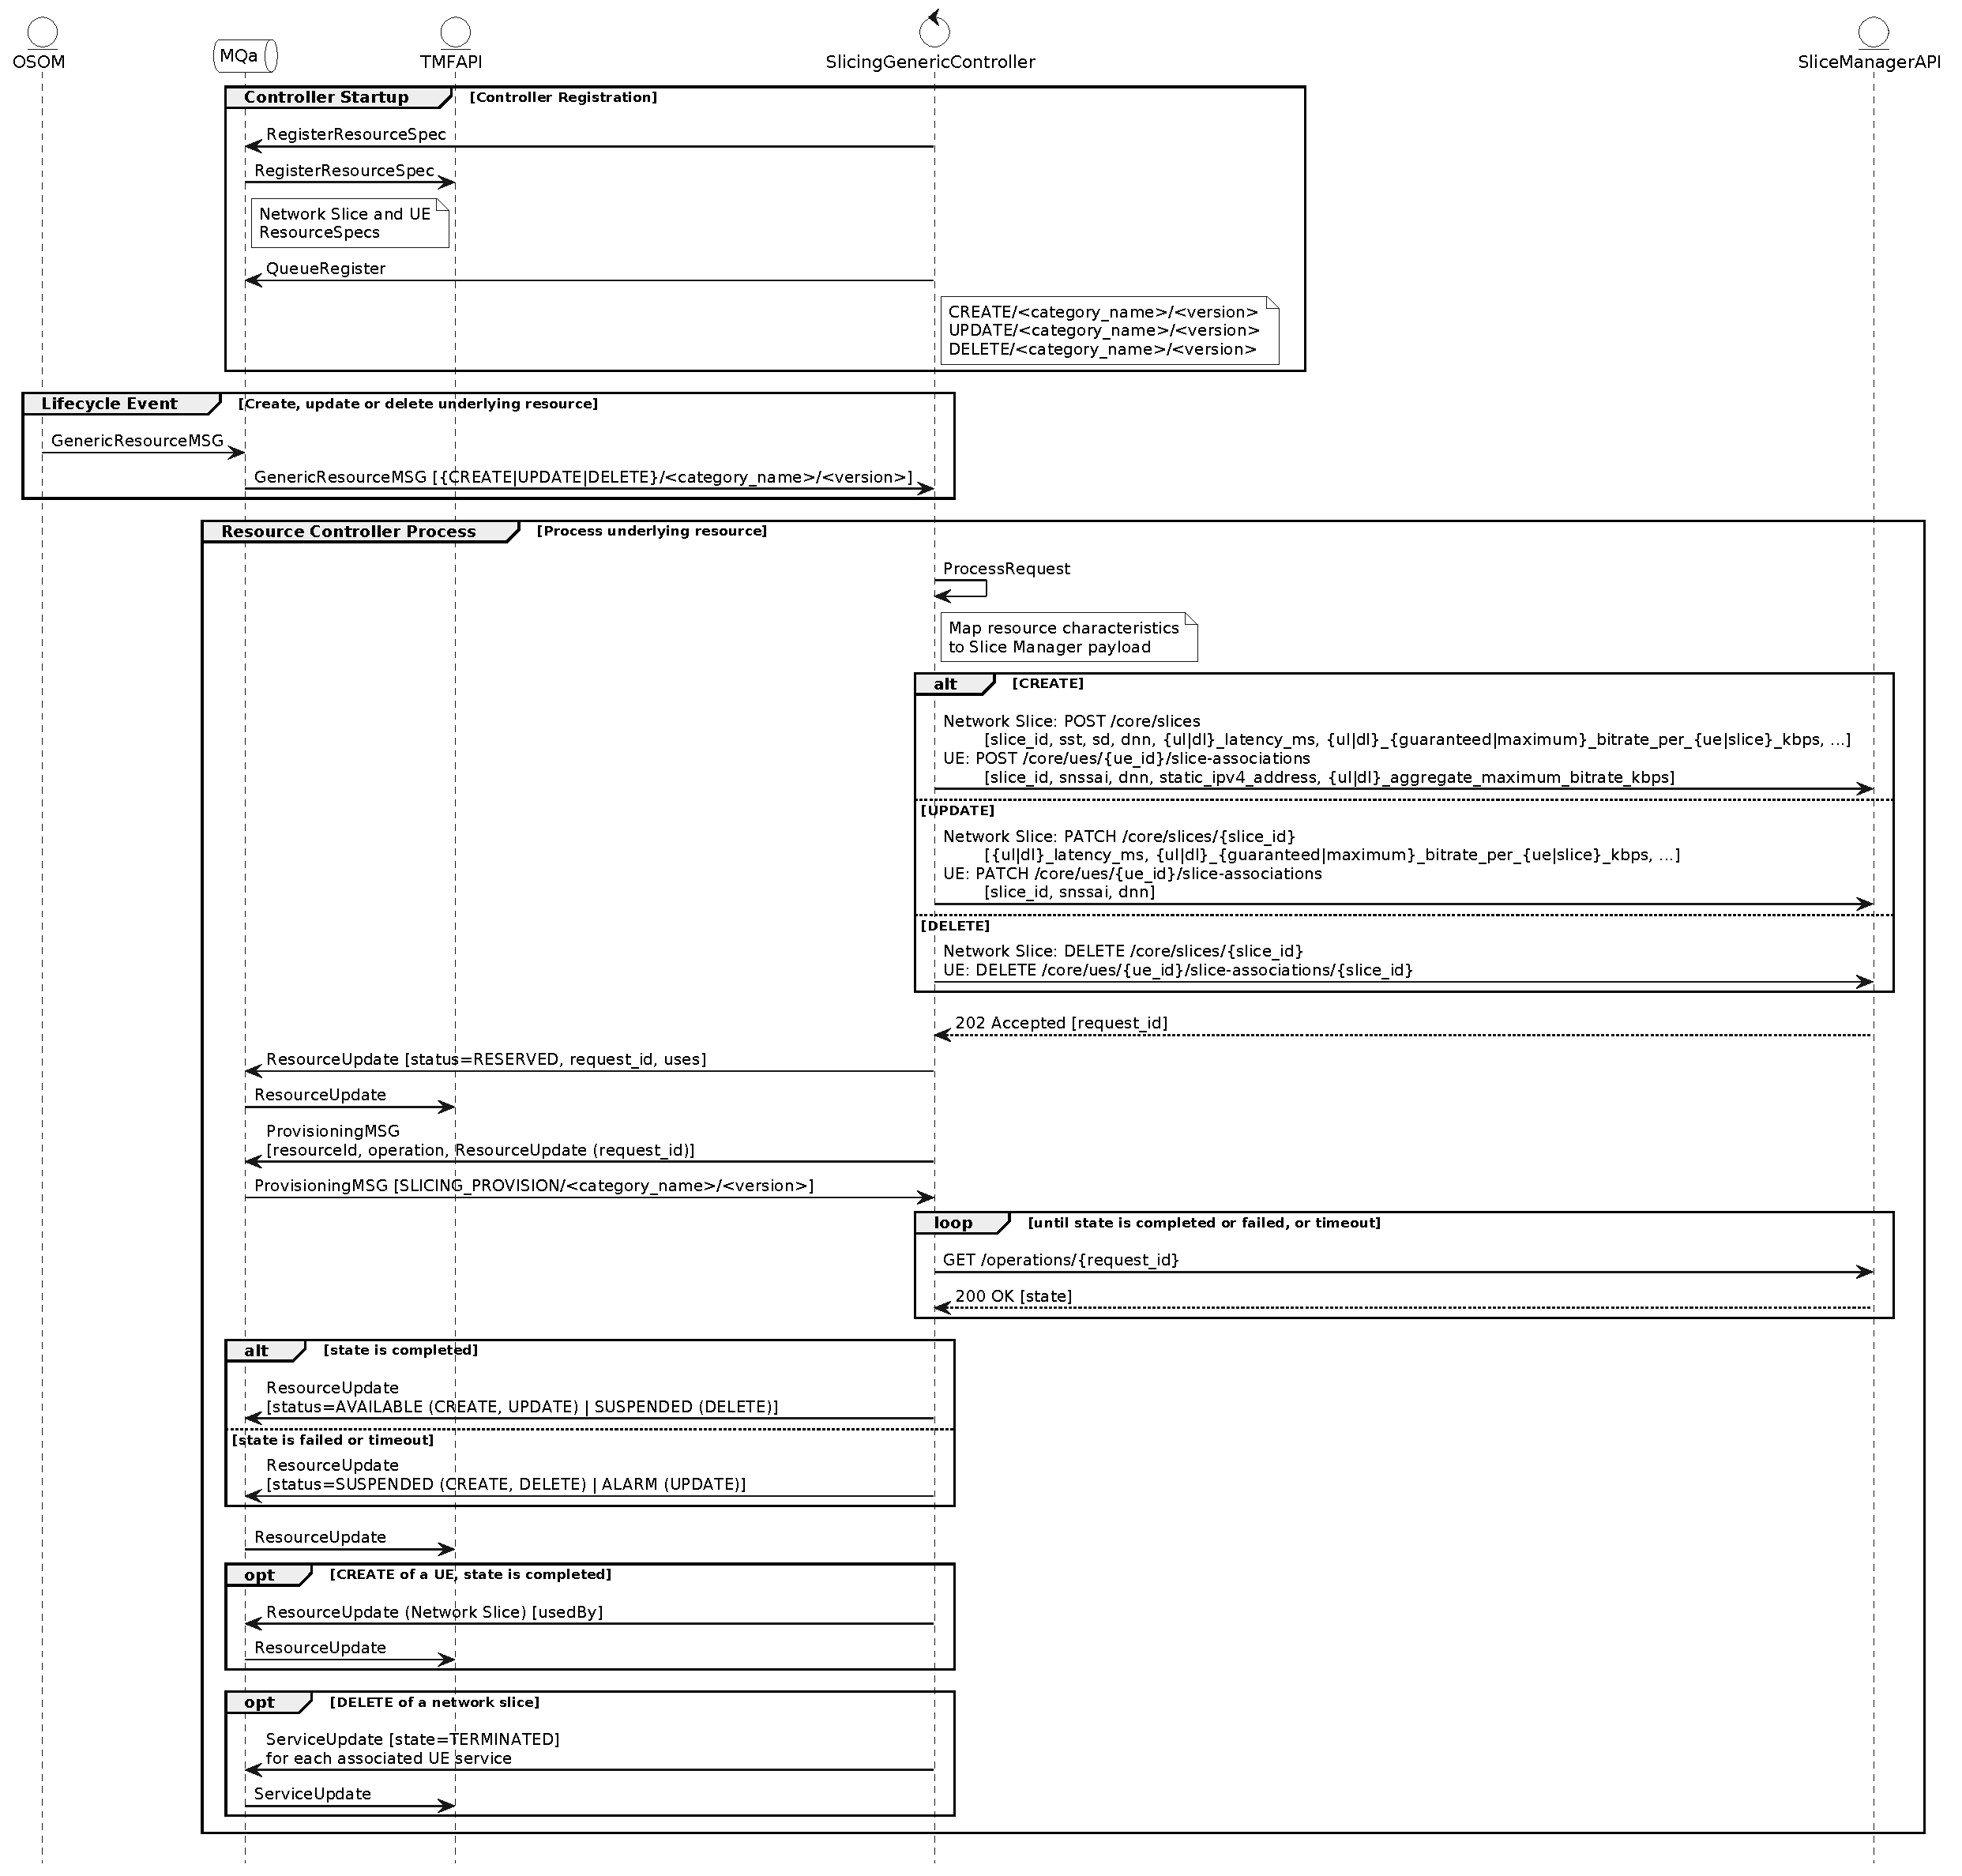
\includegraphics[width=1\linewidth]{figs/plantuml/slicing-gcontroller-lifecycle-sequence.pdf}
    \caption{Sequence Diagram for the \acs{LCM} of Network Slice and \acs{UE} Resources via the Slicing Generic Controller}
    \label{fig:impl:resource_lifecycle:flow:sequence}
\end{figure}

Before processing any lifecycle event, the controller registers with \acs{OSL} at startup (Controller Startup). Through the message queue, it registers the Network Slice and \acs{UE} Resource Specifications in \acs{OSL}, exposed by the \acs{TMF} \acsp{API}, subscribing to one separate queue per lifecycle event (\texttt{CREATE}, \texttt{UPDATE} and \texttt{DELETE}).

Each lifecycle event is delivered by OSOM to the corresponding queue, and received by the Generic Controller. The controller then maps the resource characteristics into the payload expected by the Slice Manager \acs{API}. The Slice Manager is therefore responsible for managing the lifecycle of network slices and their associations with \acsp{UE}, ensuring consistency across the various parts of the \acs{5G} system, e.g. \acs{5GC}, \acs{RAN}. In contrast, the Generic Controller serves as a synchronization layer between the \acs{OSL} \acs{TMF} resources and the state maintained by the Slice Manager.

In Figure~\ref{fig:impl:resource_lifecycle:flow:sequence}, the mapping between lifecycle events and Slice Manager endpoints is summarized in the first alternative block. A \texttt{CREATE} event results in a \texttt{POST} request to \texttt{/core/\allowbreak slices}, which provisions the network slice, or to \texttt{/core/\allowbreak ues/\allowbreak \{ue\_\allowbreak id\}/\allowbreak slice\allowbreak -associations}, which associates the \acs{UE} id, i.e. the \acs{IMSI}, with an existing slice. An \texttt{UPDATE} event results in a \texttt{PATCH} request to \texttt{/core/\allowbreak slices/\allowbreak \{slice\_\allowbreak id\}}, modifying the \acs{QoS} parameters of the slice in place while preserving its \acs{UE} associations, or to \texttt{/core/\allowbreak ues/\allowbreak \{ue\_\allowbreak id\}/\allowbreak slice\allowbreak -associations}, moving the \acs{UE} to another slice. Finally, a \texttt{DELETE} event results in a \texttt{DELETE} request to \texttt{/core/\allowbreak slices/\allowbreak \{slice\_\allowbreak id\}} or to \texttt{/core/\allowbreak ues/\allowbreak \{ue\_\allowbreak id\}/\allowbreak slice\allowbreak -associations/\allowbreak \{slice\_\allowbreak id\}}, removing the slice or the \acs{UE} association, respectively.

Throughout these operations, the Slice Manager performs the necessary interactions with the \acs{5G} System to provision or deprovision the requested resources. It is also responsible for ensuring the validity of each request, rejecting, for instance, the association of a \acs{UE} with a non-existent slice. Otherwise, the Slice Manager accepts the request with a \texttt{202 Accepted} response carrying an operation identifier (\texttt{request\_id}). The controller does not wait for the operation to complete before replying to OSOM, since OSOM treats a reply that exceeds its request timeout as a deployment failure, while the provisioning of a network slice may take considerably longer. Instead, the controller stores the operation identifier as a resource characteristic, sets the resource status to \texttt{RESERVED} through the \acs{OSL} \acs{TMF} \acsp{API}, and replies immediately.

The operation is then published to a persistent queue (\texttt{SLICING\_\allowbreak PROVISION}), scoped by the same category and version, and consumed by a dedicated polling service within the controller. Messages in this queue are only acknowledged once the final resource status is written back to \acs{OSL}, so a controller restart results in the redelivery of pending operations rather than in resources left indefinitely in the \texttt{RESERVED} state. Furthermore, messages are grouped by resource identifier, ensuring that operations targeting the same resource are processed in order, for example, preventing a deletion from overtaking the creation it cancels.

The polling service periodically queries the \texttt{/operations/\allowbreak \{request\_\allowbreak id\}} endpoint until the operation state is reported as either completed or failed, or until a predefined timeout elapses. Polling is required since the Slice Manager does not support callback endpoints. Based on the outcome, the controller updates the status of the \acs{OSL} resource, again through the \acs{TMF} \acsp{API}. Successful creations and updates set the resource to \texttt{AVAILABLE}, while successful deletions set it to \texttt{SUSPENDED}, allowing \acs{OSL} to transition the corresponding service to the \texttt{TERMINATED} state. Failed creations and deletions also set the resource to \texttt{SUSPENDED}, preventing OSOM from waiting indefinitely on an operation that will not complete. Failed updates, in turn, set the resource to \texttt{ALARM}, since the resource remains provisioned and carrying traffic, and deleting it would not revert the requested modification. In all cases, the outcome of the operation is stored as a resource characteristic, so that the result is reported back to the client through the \acs{OSL} service state.

To keep track of which \acsp{UE} are associated with each network slice, the controller also maintains relationships between the corresponding \acs{OSL} resources. Upon the creation of a \acs{UE}, a \texttt{uses} relationship referencing the target slice is added to the \acs{UE} resource, together with the \texttt{RESERVED} status, and, once the association completes, a reverse \texttt{usedBy} relationship referencing the \acs{UE} is added to the slice resource. Lastly, the deletion of a network slice implicitly removes all \acs{UE} associations in the Slice Manager. To keep the \acs{OSL} state consistent with the network, the controller sets the services of every \acs{UE} associated with the deleted slice to \texttt{TERMINATED}, which in turn triggers OSOM to send a \texttt{DELETE} message for each corresponding \acs{UE} resource and, consequently, the deletion of the resource.
